Rekapitulasi pengujian kecepatan adalah sebagai berikut:

Hasil rata-rata dari kecepatan \textit{loading} dan \textit{request} terhadap sistem adalah sebagai berikut, sesuai dengan segmentasi yang telah dipaparkan pada subbab Pengujian Kecepatan:
\begin{enumerate}
	\item \textit{DOM Loading}: 104,2 ms
	\item \textit{Scripting}: 914,6 ms
	\item \textit{Rendering}: 313,7 ms
\end{enumerate}

Visualisasi perbandingan dan komparasi antara ketiga segmentasi tersebut dapat dilihat lewat diagram batang pada Gambar \ref{diagram-pengguna-chart}.

\begin{figure}[H]
	\centering
	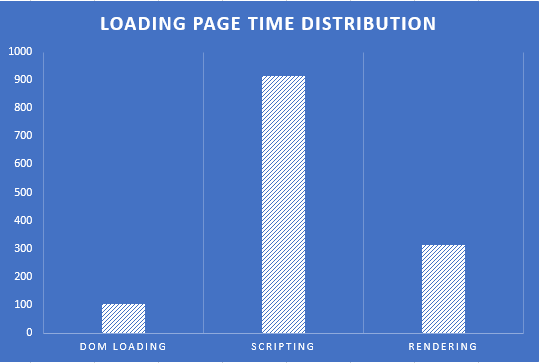
\includegraphics[width=\textwidth]{images/bab5/speed/bar-chart.png}
	\caption{Diagram batang hasil pengujian kecepatan sistem }
	\label{chart-speed-test}
\end{figure}

\begin{figure}[H]
	\centering
	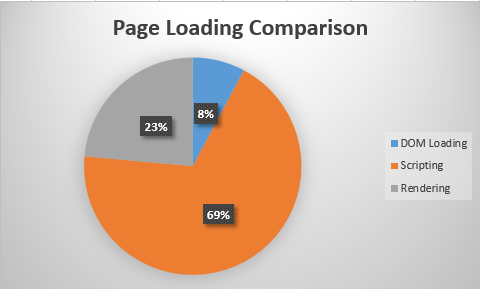
\includegraphics[width=\textwidth]{images/bab5/speed/circle-chart.png}
	\caption{Diagram lingkaran hasil pengujian kecepatan}
	\label{circle-chart-speed-test}
\end{figure}

Dari angka tersebut, dapat dilihat bahwa proses \textit{scripting} sangat memakan waktu, yang berarti konten dan \textit{assets} yang di\textit{load} dalam page cukup besar. Tampak dari waktu \textit{loading page} halaman menampilkan daftar barang mencapai waktu \textit{loading} terlama, karena pada halaman tersebut terdapat sangat banyak gambar berukuran besar dan adanya beberapa \textit{script} dibutuhkan yang kurang efisien (butuh \textit{owl-carousel}, \textit{bootstrap} untuk me\textit{load} setiap halaman). \\